\documentclass[handout]{beamer}
% Class options include: notes, notesonly, handout, trans,
%                        hidesubsections, shadesubsections,
%                        inrow, blue, red, grey, brown
\usepackage{graphicx}
\usepackage{hyperref}
\usepackage{fancyvrb}
\usepackage{subfig}

\usepackage[utf8]{inputenc}
\usepackage[spanish]{babel}
\usepackage[style=authoryear]{biblatex}
\renewcommand*{\nameyeardelim}{\addcomma\addspace}

\uselanguage{Spanish}
\languagepath{Spanish}

% Theme for beamer presentation.
\usepackage{beamerthemesplit} 
% Other themes include: beamerthemebars, beamerthemelined, 
%                       beamerthemetree, beamerthemetreebars  
% \usetheme{Warsaw}
% \usetheme{Rochester}
\usetheme{Boadilla}

\setbeamertemplate{headline}{%
\leavevmode%
  \hbox{%
    \begin{beamercolorbox}[wd=\paperwidth,ht=2.5ex,dp=1.125ex]{palette quaternary}%
    \insertsectionnavigationhorizontal{\paperwidth}{}{\hskip0pt plus1filll}
    \end{beamercolorbox}%
  }
}

\title[CeCAR]{Utilizando el CeCAR}
% \subtitle{Tesis presentada para optar al título de Doctor de la Universidad de Buenos Aires en el área Ciencias de la Computación}
\author[Saveli Vassiliev]{Saveli Vassiliev}
\institute[UBA, FCEyN, IC]{Universidad de Buenos Aires \\ Facultad de Ciencias Exactas y Naturales, Instituto de Cálculo}
\date{\today}                    % Enter the date or \today between curly braces

\begin{document}

% Creates title page of slide show using above information
\begin{frame}
  \titlepage
\end{frame}

%\section[Outline]{}
%
%% Creates table of contents slide incorporating
%% all \section and \subsection commands
%\begin{frame}
%  \tableofcontents
%\end{frame}


\begin{frame}
\frametitle{Plan}
\begin{itemize}
  \item<+-> Hoy
  \begin{itemize}
    \item CeCAR (\url{https://cecar.fcen.uba.ar/}) -- ¿de qué se trata?
    \item Creación de claves y usuarios. Usaremos \Verb=PuTTY= para conectarnos al cluster y \Verb=WinSCP= para mover archivos.
    \item Introducción a la terminal de Linux. Aplicaciones de consola que les mejorarán la vida si las aprenden a usar.
  \end{itemize}
  \item<+-> Mañana
  \begin{itemize}
    \item Introducción a comandos de control de \Verb=SLURM=.
    \item Computando $\pi$ usando \Verb=R=: enviando un trabajo, leyendo el output, mirando el estado.
  \end{itemize}
  \item<+-> Próximas dos semanas (para la gente del IC): estoy para resolver sus problemas, documentar los problemas más frecuentes y ayudarles a que todo funcione en sus aplicaciones particulares.
\end{itemize}
\end{frame}

\begin{frame}
\frametitle{CeCAR}
\textbf{Ce}ntro de \textbf{C}ómputo de \textbf{A}lto \textbf{R}endimiento

\begin{itemize}
  \item Cluster de exactas, físicamente en el pabellón 1, que tiene:
  \item $\approx 45$ nodos
  \item $\approx 90$ CPUs
  \item $\approx 700$ núcleos (cores / threads)
  \item 26 GPUs (no vamos a ver esto)
\end{itemize}
\end{frame}


\begin{frame}
\frametitle{Caso de uso: Monte Carlo}
\begin{itemize}
  \item<+-> Método: correr $n$ veces algo randomizado y hacer estadística sobre el output.
  \item<+-> Problema: cada iteración tarda mucho.
  \item<+-> Solución ``casera'': lanzamos la misma aplicación 4 veces con $n/4$ iteraciones y tardamos 4 veces menos. Inmediatamente uno piensa...
\end{itemize}
\onslide<+->
\begin{center}

\includegraphics[width=20em]{ifonly.jpg}
\end{center}
\end{frame}

\begin{frame}
\frametitle{Caso de uso: Monte Carlo}
\begin{itemize}
  \item En el IC este problema lo tiene mucha gente.
  \item Es el más fácil de resolver sin tener que ``programar en paralelo'' (i.e., sincronización, locks, memoria compartida, cuellos de botella, etc).
  \item Es lo que estaremos haciendo. Podrán ejecutar cosas con $n/100$ o $n/500$ en vez de $n/4$. 
\end{itemize}
\end{frame}


\begin{frame}
\frametitle{Workflow}
\begin{center}
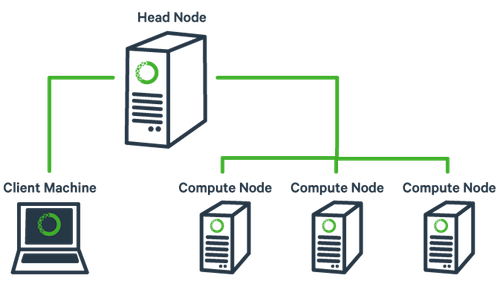
\includegraphics[width=15em]{cluster_diagram.png}
\end{center}
\begin{enumerate}
  \item Uno se conecta a un nodo ``controlador'' (\Verb=Head Node=).
  \item Le dice al scheduler los parámetros de su programa y este se encarga de usar los nódos de cómputo.
\end{enumerate}
\end{frame}

\begin{frame}
\begin{center}
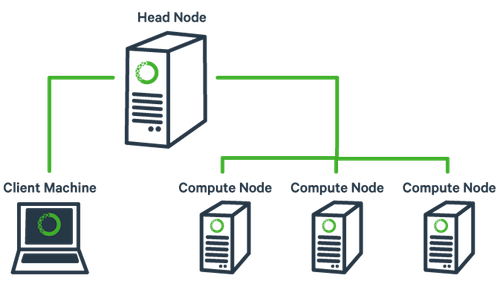
\includegraphics[width=15em]{cluster_diagram.png}
\end{center}
Salvo quizás la máquina de ustedes (\Verb=Client Machine=), todo corre Linux. Para ``hablarle'' a \Verb=SLURM= no queda otra que saber usar una consola. 
\vspace{1em}
\pause

Esto lo veremos luego de explicar como crear un usuario en el CeCAR.
\end{frame}

\begin{frame}
\frametitle{Para usuarios de Windows}
\begin{enumerate}
  \item Descargar e instalar PuTTY de \url{https://www.putty.org/}
  \item Abrir \Verb=<Archivos de programa>/puttygen.exe=
  \item Clickear en \Verb=Generate= (esto genera un par de claves, la pública y la privada).
  \item Poner un nombre que les permita recordar qué computadora usan en \Verb=Key comment= (sin espacios).
\end{enumerate}
  \begin{center}
  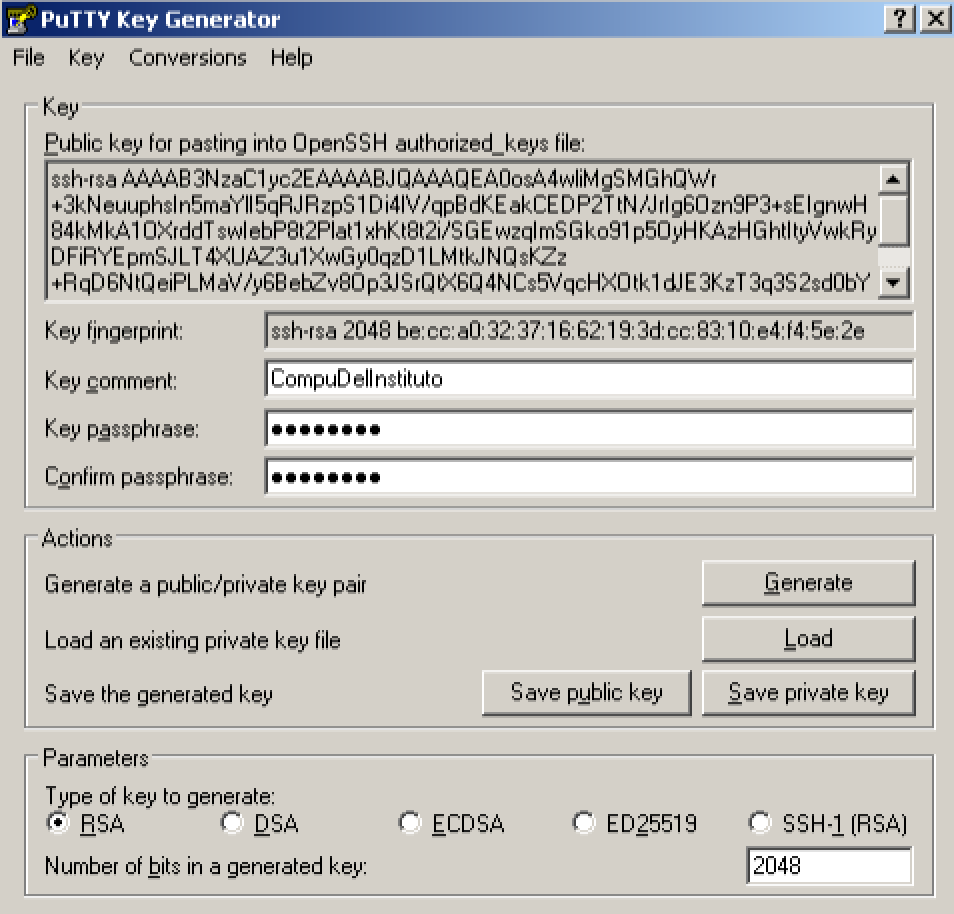
\includegraphics[width=13em]{./puttygen}
  \end{center} 
\end{frame}

\begin{frame}
\begin{enumerate}
  \item Escribir un passphrase (una contraseña suya).
  \item Guardar la clave privada en un archivo \Verb=cecar.ppk=
  \item Ir a \url{https://cecar.fcen.uba.ar/solicitud/hpc/} y completar todos los campos, copiando la clave generada como sigue.
\end{enumerate}
\begin{center}
  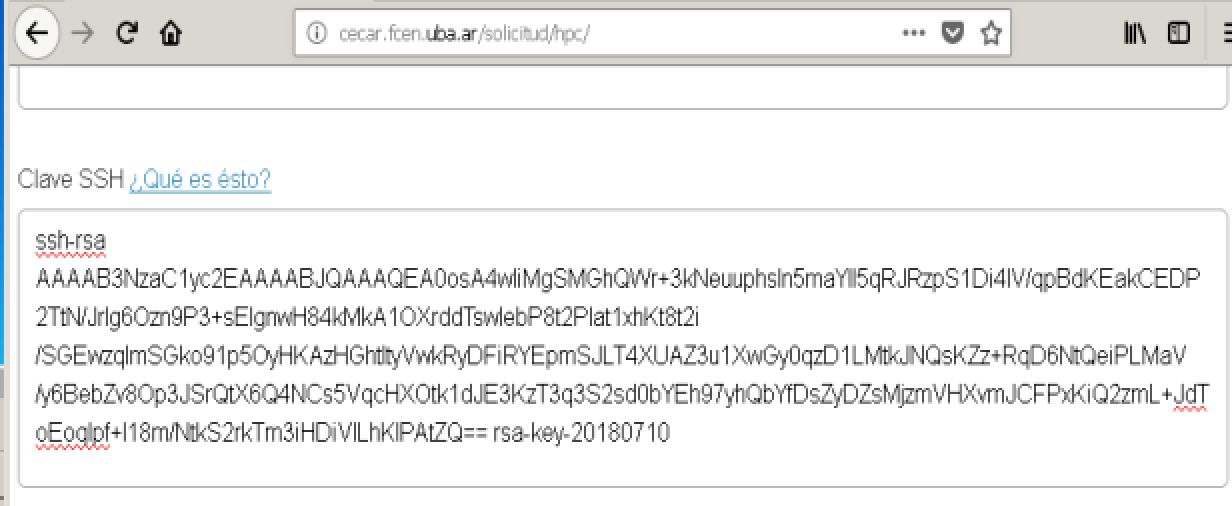
\includegraphics[width=23em]{./ssh-web-cecar}
  \end{center} 
\end{frame}

\begin{frame}
\frametitle{Usando la clave privada}
Le hacen doble click a su clave \Verb=cecar.ppk= y eso lanza un agente que les hace la autenticación cuando usen \Verb=PuTTY=.

\begin{center}

\includegraphics[width=2em]{cecarppk.png}
\end{center}

Con esto ya se pueden conectar al cluster con PuTTY:
\begin{center}
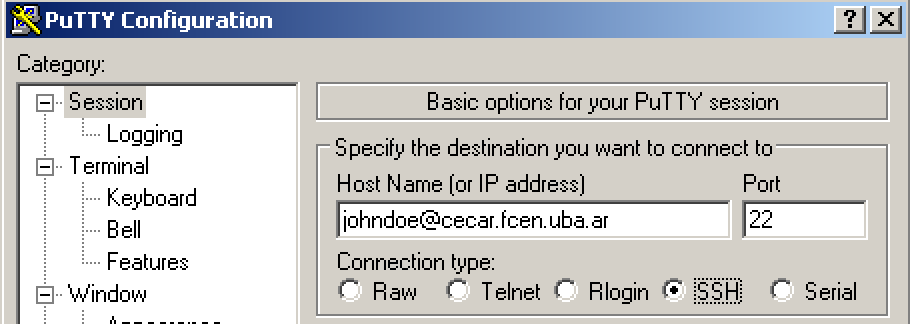
\includegraphics[width=30em]{putty-cfg.png}
\end{center}
\end{frame}

\begin{frame}
\frametitle{Usando la clave privada}
Si todo salió bien, si clickean en \Verb=Open= deberían ver algo así:
\begin{center}
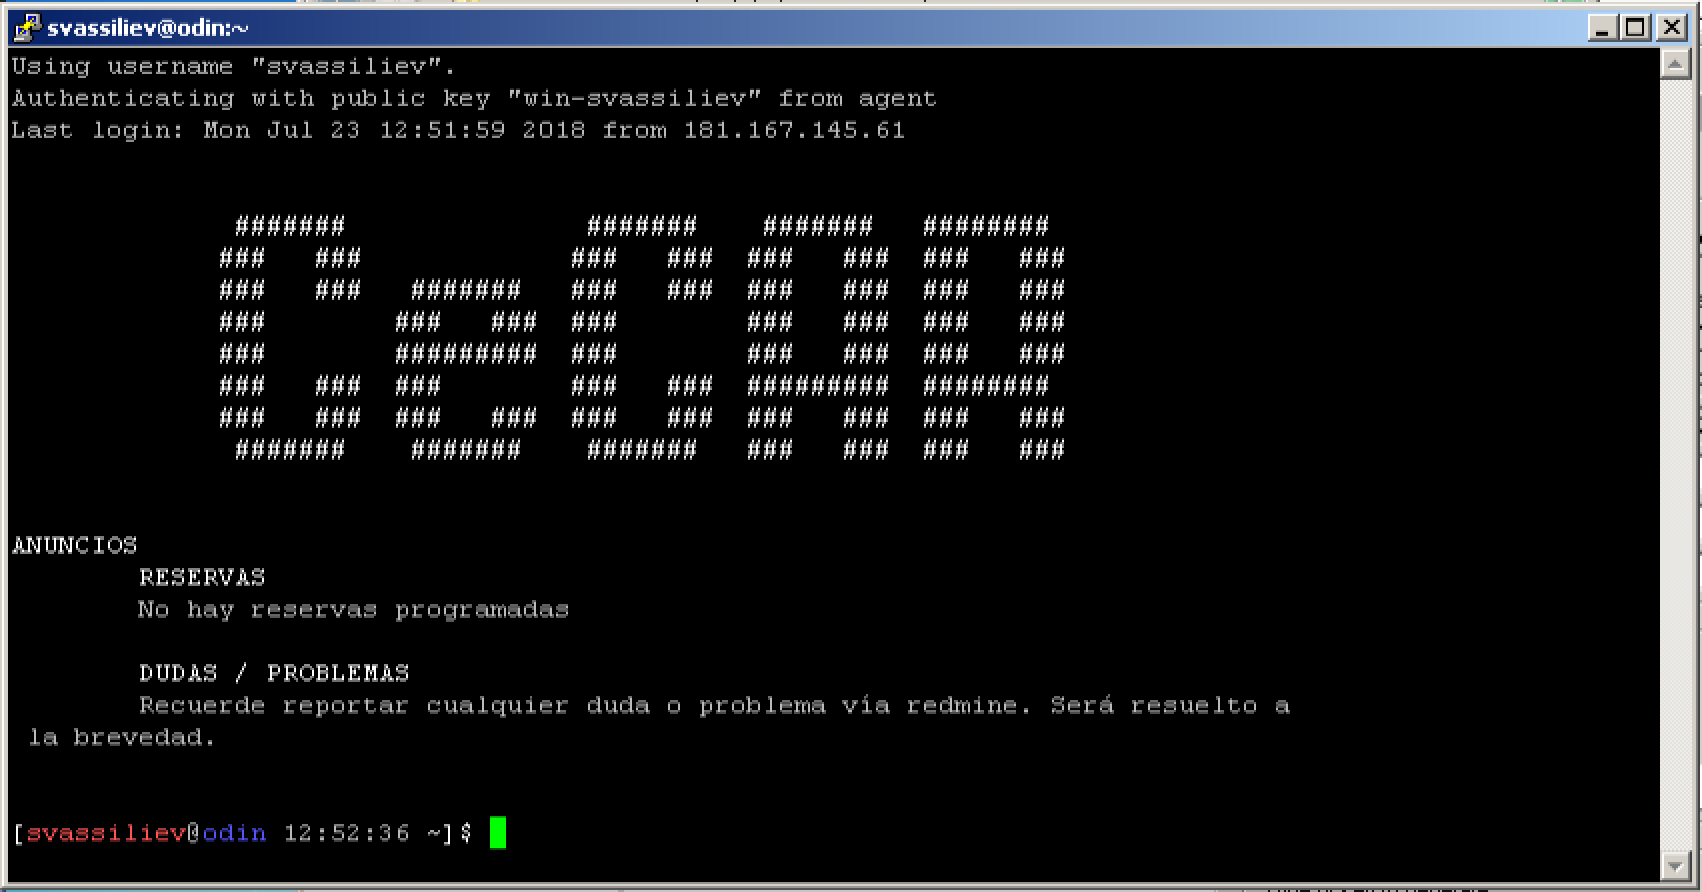
\includegraphics[width=30em]{putty-session.png}
\end{center}
\end{frame}



\begin{frame}
\frametitle{WinSCP: Moviendo archivos al cluster y de vuelta}
\begin{enumerate}
  \item Descargar e instalar \Verb=WinSCP= de \url{https://winscp.net/}
  \item Crear una nueva conexión como sigue
\end{enumerate}
\begin{center}
  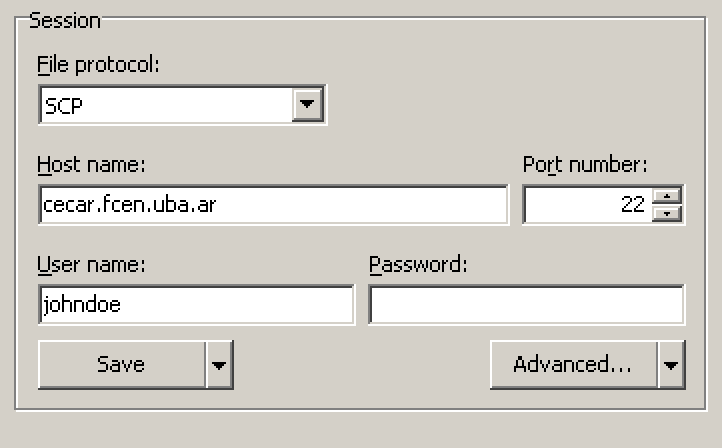
\includegraphics[width=17em]{winscp-session.png}
  \end{center} 
  Le pueden dar save y tenerlo como acceso directo. 
\end{frame}


\begin{frame}
\frametitle{WinSCP: Moviendo archivos al cluster y de vuelta}
Para usar WinSCP deben tener el agente de las claves corriendo (se abre cuando hacen doble click en \Verb=cecar.ppk=).

Si todo salió bien, debería verse así:

\begin{center}
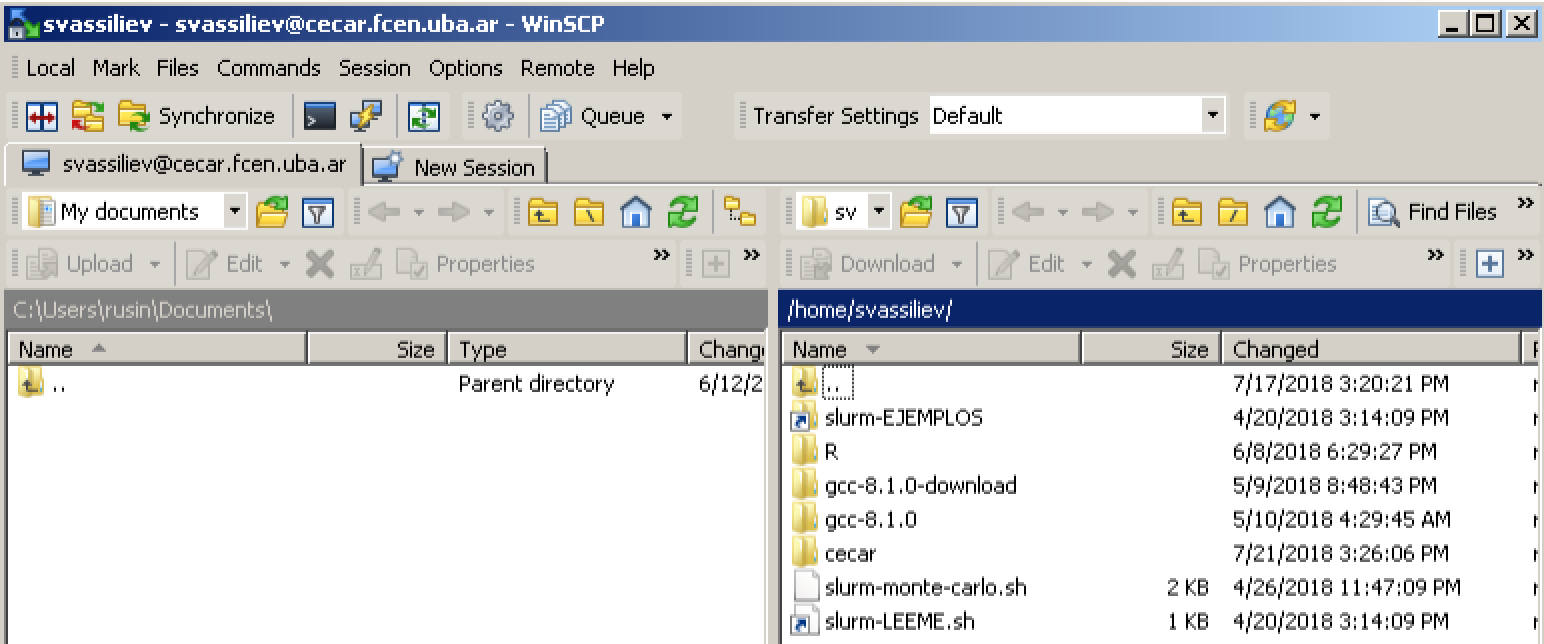
\includegraphics[width=30em]{winscp.png}
\end{center}
\end{frame}


\begin{frame}
\frametitle{Linux 101}
Para jugar un poco con Linux lo mejor es hacer una máquina virtual:

\begin{enumerate}
  \item Descargar VirtualBox de \url{https://www.virtualbox.org/wiki/Downloads} e instalarlo.
  \item Descargar un \Verb=.iso= de Ubuntu 18.04 (distro de linux linda): \url{www.ubuntu.com} - Downloads - Desktop.
  \item Crear una máquina nueva en VirtualBox e instalar el ubuntu ahí (lo hacemos en vivo).
  \end{enumerate}

\end{frame}

\begin{frame}
Desde una terminal de linux:
 \begin{itemize}
  \item ls
  \item cd
  \item cp
  \item man
  \item mv
  \item rm
  \item cat
  \item less
  \item sh
  \item redirigiendo stdout
  \item vim
 \end{itemize}
\end{frame}

\begin{frame}
\huge{Mañana haremos uso de todo esto!\\A crear usuarios e instalar todo!}

\huge{Gracias!}
\end{frame}



\end{document}